%%%%%%%%%%%%%%%%%%%%%%%%%%%%%%%%%%%%%%%%%
% Stylish Article
% LaTeX Template
% Version 1.0 (31/1/13)
%
% This template has been downloaded from:
% http://www.LaTeXTemplates.com
%
% Original author:
% Mathias Legrand (legrand.mathias@gmail.com)
%
% License:
% CC BY-NC-SA 3.0 (http://creativecommons.org/licenses/by-nc-sa/3.0/)
%
%%%%%%%%%%%%%%%%%%%%%%%%%%%%%%%%%%%%%%%%%

%----------------------------------------------------------------------------------------
%	PACKAGES AND OTHER DOCUMENT CONFIGURATIONS
%----------------------------------------------------------------------------------------

\documentclass[fleqn,10pt,ngerman]{SelfArx}
\usepackage{babel}
\selectlanguage{ngerman}

\setlength{\columnsep}{0.55cm} % Distance between the two columns of text
\setlength{\fboxrule}{0.75pt} % Width of the border around the abstract

\definecolor{color1}{RGB}{0,0,90} % Color of the article title and sections
\definecolor{color2}{RGB}{0,20,20} % Color of the boxes behind the abstract and headings

\newlength{\tocsep} 
\setlength\tocsep{1.5pc} % Sets the indentation of the sections in the table of contents
\setcounter{tocdepth}{2} % Show only three levels in the table of contents section: sections, subsections and subsubsections

\usepackage{comment}

\usepackage{fontenc}
\usepackage{inputenc}
\usepackage{url} 
\usepackage{hyperref}
\usepackage{listings}

%----------------------------------------------------------------------------------------
%	ARTICLE INFORMATION
%----------------------------------------------------------------------------------------

\JournalInfo{Software-Technik-Praktikum} % Journal information
\Archive{Sommersemester 2019} % Additional notes (e.g. copyright, DOI, review/research article)

\PaperTitle{Implementierung von REST Services zur Umsetzung der SQLcoach Anwendung} % Article title

\Authors{Max Mustermann} % Authors
\affiliation{\textit{Hochschule Kaiserslautern}} % Author affiliation
\affiliation{\textbf{Corresponding author}: max.mustermann@hs-kl.de} % Corresponding author

\Keywords{SQL-Coach, REST, Java, Service} % Keywords - if you don't want any simply remove all the text between the curly brackets
\newcommand{\keywordname}{Keywords} % Defines the keywords heading name

%----------------------------------------------------------------------------------------
%	ABSTRACT
%----------------------------------------------------------------------------------------

\Abstract{Das Abstract ist eine maximal 200 Worte lange Zusammenfassung des Inhalts der Arbeit, so dass sich der Leser vorab ein erstes Bild vom Inhalt machen kann.}

%----------------------------------------------------------------------------------------

\begin{document}
	
	\flushbottom % Makes all text pages the same height
	
	\maketitle % Print the title and abstract box
	
	\tableofcontents % Print the contents section
	
	\thispagestyle{empty} % Removes page numbering from the first page
	
	%----------------------------------------------------------------------------------------
	%	ARTICLE CONTENTS
	%----------------------------------------------------------------------------------------
	
	\section*{Anforderungen}
	Entfernen Sie bitte diesen Abschnitt aus Ihrem fertigen Dokument und arbeiten Sie den Inhalt in den Text mit ein. 
	Ihr REST Service soll folgende User Stories abdecken.
	
	\begin{enumerate}
		
		\item Der REST-Service liefert auf Anfrage alle Szenarien mit allen Infos zu den Szenarien. 
		\item  Der REST-Service liefert auf Anfrage alle Aufgabengruppen zu einem Szenario mit allen Infos zu den Gruppen. 
		\item  Der REST-Service liefert auf Anfrage alle Aufgaben zu einer Aufgabengruppe mit allen Infos zu den Aufgaben. 
		\item  Der REST-Service erlaubt das Hinzufügen von Szenarien, Aufgabengruppen und Aufgaben.
		\item  Der REST-Service erlaubt das Ändern der Eigenschafen zu Szenarien, Aufgabengruppen und Aufgaben.
		\item  Der REST-Service erlaubt das Löschen von Szenarien, Aufgabengruppen und Aufgaben.
		\item  Der REST-Service erlaubt das Anlegen, Ändern und Löschen von Trainingsdatensätzen mit frei konfigurierbaren Datasources.
		\item  Der REST-Service erlaubt das Auslesen der Tabelleninformation aller Tabellen in einem Trainingsdatensatz (Tabelleninformation = Tabellennamen, Spaltennamen, Prim\"arschl\"ussel, Sekund\"arschl\"ussel).
		\item  Der REST-Service erlaubt das ausf\"uhrung von beliebigen 
		\textit{SELECT} Abfragen auf den Trainingsdatens\"atzen.
		\item Der Personaldatensatz von Prof. Schiefer muss mit eingebunden werden, so dass Ihr Service nach der Installation sofort einsatzbereit ist. 	
		
		
	\end{enumerate}
	
	
	Weitere Anforderungen:
	\begin{enumerate}
		
		\item Voll dokumentierter Quellcode (jede \textit{PUBLIC} Klasse und Methode hat sinnvollen JavaDoc)
		\item Guter Programmierstil (insb. Namensgebung, Funktionen, Objekte, Exceptions, Logging usw.)
		\item Zero Warnings bei SonarJava oder Intellij Code Inspection (oder Argumentation warum diese Warnung ignoriert werden kann)
		\item Exakte Einhaltung der vorgegebenen REST Schnittstellen
		\item Exakte Einhaltung der vorgegebenen maven/ docker Installation
		\item Trainingsdatens\"atze in einer von den Stammdaten unabhängiger Postgres Instanz (innerhalb von Docker). 
		\item Nachvollziehbare Branches in Ihrem GIT (Namenskonvention: SCS-[NUM]-[feature/ bugfix /doc/ refact/ test]-name) 
		
	\end{enumerate}
	
	
	\section{Einleitung} % The \section*{} command stops section numbering
	
	\addcontentsline{toc}{section}{\hspace*{-\tocsep}Einleitung} 
	
	Die Einleitung sollte ausreichenden Hintergrund für den Leser liefern, so dass er sich ohne großes Studium von Sekundärliteratur in das Thema hineindenken kann. 
	
	Es sollen hier die grundlegenden fachlichen Begriffe eingeführt werden. 
	
	Auch sollte die Motivation für die vorliegende Arbeit dargelegt werden, sowie die Zielsetzung, die man erreichen will. Weiter wird auch das Thema von eventuell verwandten Themen abgegrenzt. Hier kann auch die Literatur \cite{Harel:1987,Harel2006,Gurp99onthe} vorgestellt werden.
	
	Als Beispiel können Sie hier ein Bild des SQLCoaches einbinden (Abbildung \ref{fig:fsm1}).
	
	\begin{figure}[ht]\centering
		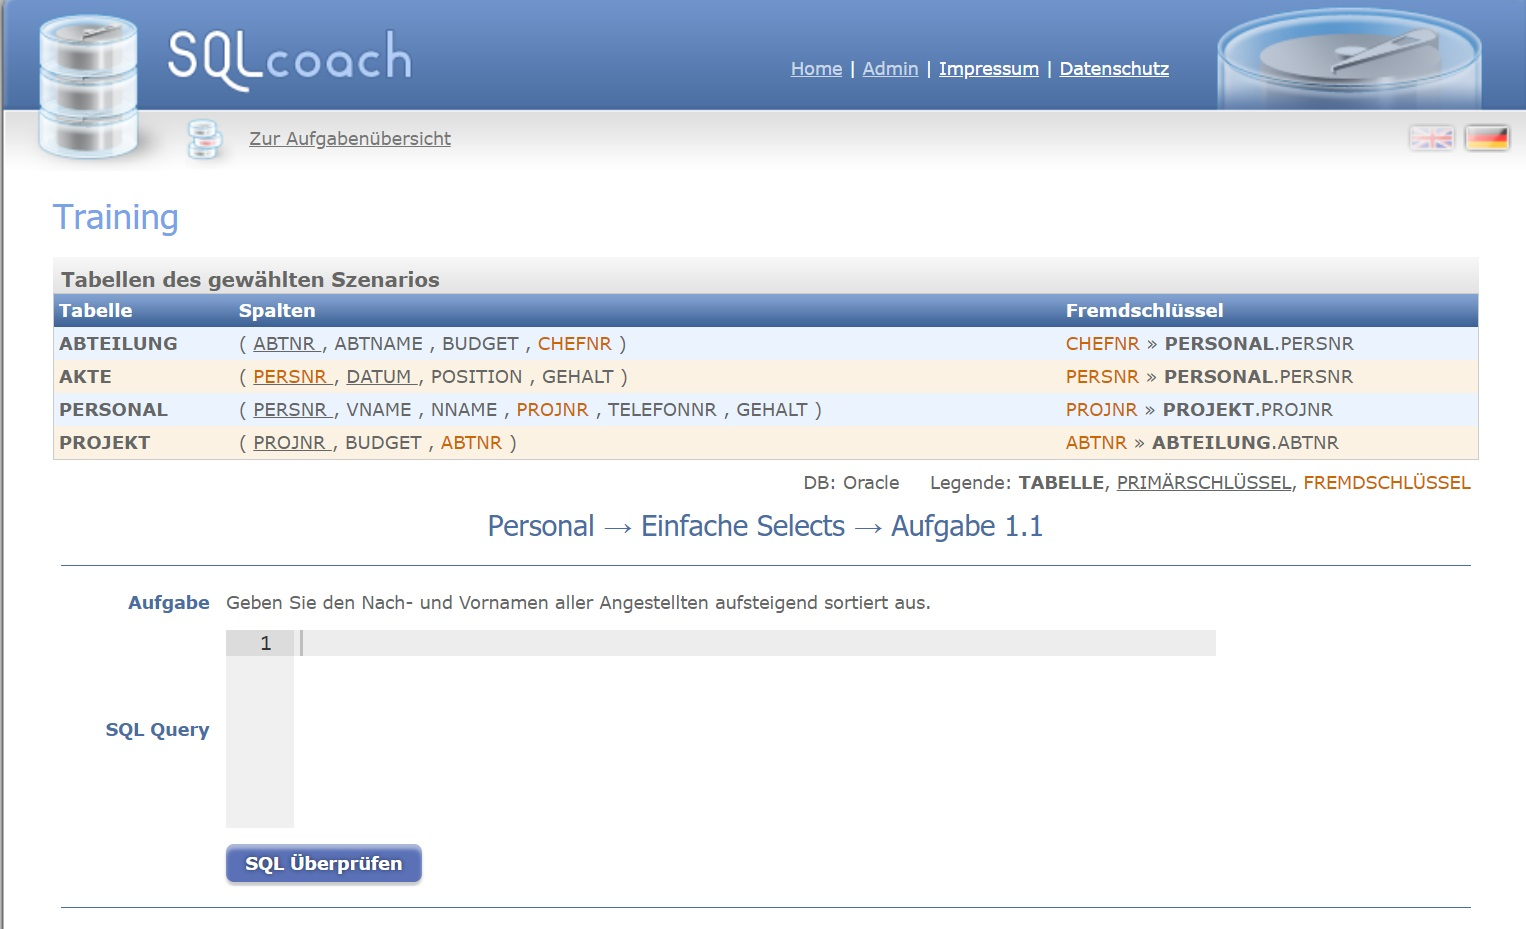
\includegraphics[width=5 cm]{Abbildungen/sqlcoach.jpg}
		\caption{Die SQLcoach Anwendung (Quelle \url{https://sqlcoach.informatik.hs-kl.de/sqlcoach/}).}
		\label{fig:fsm1}
	\end{figure}
	
	Folgende Punkte könnten hier angesprochen werden:
	\begin{itemize}[noitemsep]
		\item Sinn und Zweck der Anwendung SQLCoach.
		\item Sinn und Zweck von REST Services.
		\item Einf\"uren der wichtigen Begriffe.
		\item Welche Problemstellung wird hier bearbeitet?
	\end{itemize}
	
	
	
	%------------------------------------------------
	
	
	
	
	
	
	
	%------------------------------------------------
	
	\section{Methoden und Werkzeuge}
	\label{sec:methoden}
	Kurze Einführung in den Abschnitt. Es wird beschrieben was jetzt kommt, d.h. welche Methoden und Werkzeuge im folgenden vorgestellt werden. 
	Es wird noch nicht darauf eingegangen was im Ganzen damit gebaut wurde. Es werden nur die Details zu den einzelnen Werkzeugen angegeben, so dass im nächsten Kapitel darauf Bezug genommen werden kann. 
	
	
	\subsection{JAX-RS}
	JAX-RS wurde im Zuge der Tutorialreihe "REST Web Services" als Java Programmierschnittstelle kennengelernt.
	Verschiedene Annotationen von JAX-RS wurden verwendet. Pfad Annotationen, welche die Url der Schnittstelle definieren, der Requesttyp, welcher die Art der Anfrage definiert, sowie @Consumes und @Poduces, welche die MIME-Typ der jeweiligen akzeptierten bzw. zurückgegebenen Ressource definieren.
	Wie wurde von dieser Technologie verwendet?
	Welche technischen Artefakte (Dateinamen, Konfiguration, Klassen,...) sind entstanden, wie heißen diese und was machen diese. 
	
	
	\subsection{Docker}
	Zwei Sätze zur Einführung der Technologie. 
	Was wurde von dieser Technologie verwendet?
	Wie wurde von dieser Technologie verwendet?
	Welche technischen Artefakte (Dateinamen, Konfiguration, Klassen,...) sind entstanden, wie heißen diese und was machen diese. 
	
	\subsection{Maven}
	Zwei Sätze zur Einführung der Technologie. 
	Was wurde von dieser Technologie verwendet?
	Wie wurde von dieser Technologie verwendet?
	Welche technischen Artefakte (Dateinamen, Konfiguration, Klassen,...) sind entstanden, wie heißen diese und was machen diese. 
	
	\subsection{Postgres}
	Zwei Sätze zur Einführung der Technologie. 
	Was wurde von dieser Technologie verwendet?
	Wie wurde von dieser Technologie verwendet?
	Welche technischen Artefakte (Dateinamen, Konfiguration, Klassen,...) sind entstanden, wie heißen diese und was machen diese. 
	
	
	\subsection{Apache Log4j}
	Zwei Sätze zur Einführung der Technologie. 
	Was wurde von dieser Technologie verwendet?
	Wie wurde von dieser Technologie verwendet?
	Welche technischen Artefakte (Dateinamen, Konfiguration, Klassen,...) sind entstanden, wie heißen diese und was machen diese. 
	
	\subsection{GIT}
	Zwei Sätze zur Einführung der Technologie. 
	Was wurde von dieser Technologie verwendet?
	Wie wurde von dieser Technologie verwendet?
	Welche technischen Artefakte (Dateinamen, Konfiguration, Klassen,...) sind entstanden, wie heißen diese und was machen diese. 
	
	
	
	\section{Ergebnisse}
	
	In diesem Abschnitt beschreiben Sie nun das Endergebnis Ihrer Arbeit. 
	%Endergebnisse beschreiben und Bezug auf Kap 2 nehmen
	%neutral nüchtern
	%passive nicht "iich habe oder wir haben" sondern " es wurde"
	\subsection{Architektur}
	
	Die beziehen sich hier auf die im Methodenteil vorgestellten Artefakte und beschreiben wie diese zusammengesetzt wurden. Welche Komponenten ruft welche Komponente auf? 
	
	\textbf{{Sie müssen hier auf jede der Methoden in Abschnitt} \ref{sec:methoden} Bezug nehmen.}
	
	
	\subsection{REST Schnittellen}
	Bitte beschreiben Sie hier auch die von Ihrer Komponenten bereitgestellten REST Schnittstellen, da diese das Endergebnis Ihrer Arbeit darstellt. 
	
	\subsection{Installation}
	Geben Sie hier eine Installationsanleitung. Ihre Software muss Sie wie folgt bauen und starten lassen: 
	
	\begin{lstlisting}
	git clone MYREPO
	
	mvn clean package
	
	docker-compose  build 
	
	docker-compose  up
	\end{lstlisting}
	
	
	%------------------------------------------------
	
	\section{Diskussion}
	
	In diesem Abschnitt werfen Sie einen kritischen Blick auf Ihre Arbeit:
	%
	\begin{enumerate}
		\item Haben Sie alle angeforderten User Stories umgesetzt? 
		\item Welche Features haben sie zus\"atzlich umgesetzt?
		\item Welche positiven Eigenschaften hat Ihre Implementierung?
		\item Welche negativen Eigenschaften hat Ihre Implementierung? 		
		\item Sind die Schnittstellen gut gelungen? Warum Sind das gute Schnittstellen? 
		\item Wie performant ist Ihre Implementierung?
		\item Welche Best Practices haben Sie eingehalten? 
		\item Wie hoch ist Ihre Test Coverage (JUnit)? 
		\item Wie ist die Code-Qualität? Berichten Sie hier über das Ergebnis der Code-Inspection (SonarJava oder IntelliJ IDEA Code-Inspection). 
	\end{enumerate}
	
	Dieser Abschnitt ist nicht leicht zu schreiben, aber dieser Abschnitt ist essentiell für Ihre Benotung. \textbf{Sie müssen hier das Positive herauszustellen!} Zudem sollen Sie hier auch auf Unzul\"anglichkeiten Ihrer Arbeit eingehen. Wenn Sie die Schwachstellen Ihrer Arbeit hier bel\"auchten und idealerweise Argumente finden warum das so gelöst wurde, dann hat einen sehr positiven Einfluss auf die Benotung. 
	
	
	
	\section{Zusammenfassung}
	Hier wird nochmal der Inhalt und die Ergebnisse der Arbeit kurz zusammen gefasst. Des Weiteren werden Themen und Aufgabenstellungen genannt, die es lohnt weiter zu untersuchen.
	
	%----------------------------------------------------------------------------------------
	%	REFERENCE LIST
	%----------------------------------------------------------------------------------------
	
	\bibliographystyle{unsrt}
	\bibliography{Literatur}
	
	%----------------------------------------------------------------------------------------
	
	\subsubsection*{Erklärung zur Ausarbeitung}
	Hiermit erkläre ich, Daniel Braun(880335), dass ich die vorliegende Ausarbeitung selbstständig und ohne fremde Hilfe angefertigt habe und keine anderen als in der Abhandlung angegebenen Hilfen benutzt habe; dass ich die Übernahme wörtlicher Zitate aus der Literatur sowie die Verwendung der Gedanken anderer Autoren an den entsprechenden Stellen innerhalb der Arbeit gekennzeichnet habe. Ich bin mir bewusst, dass eine falsche Erklärung rechtliche Folgen haben kann.\\ \\
	--------------------- \\
	Unterschrift
	
	
\end{document}